\documentclass[12pt,a4paper]{cibb}

% Fallback definition for missing \@ordinalM
\makeatletter
\providecommand{\@ordinalM}[2]{#1}
\makeatother

\usepackage{subfigure,graphicx}
\usepackage{amsmath,amsfonts,latexsym,amssymb,euscript,xr}
\usepackage{booktabs}
\usepackage[nodayofweek]{datetime}
\usepackage{hyperref}
\usepackage{fmtcount}
\usepackage[english]{datenumber}
\usepackage[absolute]{textpos}



\usepackage[table]{xcolor}
\usepackage{color,colortbl,tabularx}

\usepackage[english]{babel}
\usepackage[protrusion=true,expansion=true]{microtype}
\usepackage{amsmath,amsfonts,amsthm}
% \usepackage[pdftex]{graphicx}
\usepackage{pifont}

\def\red{\color{red}}
\def\black{\color{black}}
\def\blue{\color{blue}}
\def\magenta{\color{magenta}}



\definecolor{LightBlue}{rgb}{0.88,0.9,0.9}

\newcommand\blfootnote[1]{%
  \begingroup
  \renewcommand\thefootnote{}\footnote{#1}%
  \addtocounter{footnote}{-1}%
  \endgroup
}

\title{\Large $\ $\\ \bf PID Control for Vehicle Lateral Dynamics}

\author{\large L.A. Torres-Romero$^1$}
\address{\footnotesize $\ $\\$^1$ DESI, ITESO,
Tlaquepaque Jalisco, Mexico. \\
%
%
\bigskip
ORCID code: 0000-0001-7632-179X.
\bigskip
\newline
$^*$corresponding author: luisarturo.torres7@gmail.com
\bigskip
\newline
}


\abstract{\small  PID control, Lateral dynamics, Error feedback. \normalsize

This work presents a PID-based implementation for vehicle lateral dynamics control, intended as a simple reference model for path tracking and controller comparison studies.
}

\begin{document}

\renewcommand{\thefootnote}{}
\footnotetext{\small{Article version: \datedate $\;$ h\currenttime  $\;$ CET}}


\thispagestyle{myheadings}
\pagestyle{myheadings}
\markright{\tt Vehicle Dynamics and Control Simulation Playground}%check year


\section{Introduction} \label{sec:Introduction}

Autonomous driving and advanced driver assistance systems require reliable lateral control strategies to ensure vehicle stability and accurate path tracking. Among the different control approaches available, PID control provides a simple and practical solution due to its ease of implementation and tuning. This work presents a PID controller for vehicle lateral dynamics using the lateral position and orientation errors. The proposed implementation is intended as a straightforward reference model that can be used for educational purposes, benchmarking against more advanced controllers, and rapid simulation studies in vehicle dynamics applications.

\section{Lateral Model Symbols} \label{sec:Symbols}

This section describes the symbols used in equations. This is based on the lateral dynamics model described in \cite{rajamani2011vehicle}, that is a linearized model of the error respect the center of the lane of the road. For more details, you can see the lateral dynamics block documentation. The symbols are as follows:
\begin{enumerate}
     \item	\(V\): Velocity of the vehicle.
     \item	\(V_x\): This is the longitudinal velocity.
     \item	\(\beta\) : Slip angle. This is the angle that makes V and the longitudinal axis of the vehicle.
     \item	\(\psi\): Heading angle (yaw angle).
     \item	\(\gamma\): \(\psi+ \beta\), this is the angle between V and the X axis of the inertial reference frame, and it is called “the course angle”.
     \item	\(\delta\): Front steer angle.
     \item	\(l_f,l_r\): Distances from the center of gravity to the front and rear axis of the vehicle.
     \item	\(L= l_f+l_r\)
     \item	\(C_{\alpha r}, C_{\alpha f}\): Cornering stiffness of rear and front wheels. The cornering stiffness is the ability of the tire to resist deformation while the vehicle is cornering.
     \item	\(I_z\): This is the momentum of inertia of the vehicle respecting the z axis.
     \item   \(m\): Mass of the vehicle.
     \item  \(g\): Gravitational acceleration.
\end{enumerate}


\section{PID Control for Lateral Dynamics}

Based on the error model for the lateral dynamics described in \cite{rajamani2011vehicle} and recalling the Ackerman’s formula for the system \(\dot{\textbf{X}} =\textbf{A}\textbf{X}+\textbf{B}u\) where u would be our \(\delta\) and $\textbf{X} $ = $ [x_1\ x_2\   x_3\ x_4] $ = $ [e_1\ \dot{e}_1\ e_2\ \dot{e}_2]$ where the errors are 
\begin{itemize}
  \item $e_1$: lateral error.
  \item $\dot{e}_1$: rate of lateral error.
  \item $e_2$: yaw rate error.
  \item $\dot{e}_2$: rate of yaw rate error.
\end{itemize}


Using the errors $e_1$ and $e_2$ as feedback signals, we can design a PID controller to compute the steering control input $u$ that will help the vehicle to track the desired path.

\begin{itemize}
  \item $e_1$: lateral error with respect to the center of the lane.
  \item $e_2$: orientation error with respect to the lane direction.
\end{itemize}

The controller uses the sum of the normalized lateral and orientation errors. The lateral error $e_1$ is normalized considering 12 ft (3.6576 m) as the maximum expected error, while the orientation error $e_2$ is normalized considering $\pi$ radians as the maximum error.

The PID controller is defined as:

\begin{equation} \label{eq:ctrl_PID}
\dot{\delta}_{ref} = \dot{u} =  K_{p}e_{pid} + K_{i}\int{e_{pid}} + K_{d}\dot{e}_{pid}
\end{equation}

where

\begin{equation}
 e_{pid} = \frac{e_{1}}{3.6576} + \frac{e_{2}}{\pi}
\end{equation}

and the controller gains are:

\begin{equation}
K_{p} = -10.4366715621745
\end{equation}

\begin{equation}
K_{i} = -1.38825323496777
\end{equation}

\begin{equation}
K_{d} = 1.48027109324461
\end{equation}

These values were obtained using the auto-tune tool of Simulink.

The Matlab block with the interface is shown in Fig. \ref{fig:PIDCtrlBlock}.


\section{PID Simulink Block}
\label{sec:Simulink}

The implementation of the PID controller is done in a Simulink block that can be used as a reference for other implementations. The block has the following interface:

\begin{itemize}
  \item \textbf{Input 1}: \textbf{E}, The state vector \textbf{X} = $[e_1\ \dot{e}_1\ e_2\ \dot{e}_2]$ that contains the lateral error, the rate of lateral error, the orientation error, and the rate of orientation error, respectively.
  \item \textbf{Input 2}: \textbf{Vx}, The longitudinal velocity of the vehicle.
  \item \textbf{Output}: The steering control law $u$ as calculated in (\ref{eq:ctrl_PID}).
\end{itemize}

\begin{figure}[ht]
	\centering
	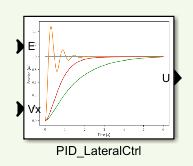
\includegraphics[width=0.4\textwidth]{./images/PID_Block.png}
	\caption{PID controller block.}
	\label{fig:PIDCtrlBlock}
\end{figure}

\section{Results}
\label{sec:RESULTS}

Figure \ref{fig:imgPID/ErrorBLDC23msNoise} shows the error in $e_1$ (distance to the lane center) and $e_2$ (orientation error). It can be observed that the lateral error reaches values up to 13 m.

Additionally, Fig. \ref{fig:imgPID/PathBLDC23msNoise} shows that the controller completely loses the trajectory and never converges back to the desired path.

\section{Conclusion}
\label{sec:CONCLUSIONS}

The PID controller provides a simple approach for lateral vehicle control using lateral and orientation errors as feedback signals. However, the simulation results show that the selected gains are not sufficient to guarantee stable path tracking under the evaluated conditions, since the vehicle diverges from the desired trajectory. More advanced control techniques or improved tuning strategies may be required to achieve robust lateral control performance.


\footnotesize
\bibliographystyle{unsrt}
\bibliography{bibliography_CIBB_file.bib} 
\normalsize

\end{document}
